\documentclass[12pt]{article}

\usepackage{amsmath, mathtools}
\usepackage{amsfonts}
\usepackage{amssymb}
\usepackage{graphicx}
\usepackage{colortbl}
\usepackage{xr}
\usepackage{hyperref}
\usepackage{longtable}
\usepackage{xfrac}
\usepackage{tabularx}
\usepackage{float}
\usepackage{booktabs}
\usepackage{caption}
\usepackage{pdflscape}
\usepackage{afterpage}

\usepackage[round]{natbib}

\hypersetup{
    bookmarks=true,         % show bookmarks bar?
    colorlinks=true,       % false: boxed links; true: colored links
    linkcolor=red,          % color of internal links (change box color with linkbordercolor)
    citecolor=green,        % color of links to bibliography
    filecolor=magenta,      % color of file links
    urlcolor=cyan           % color of external links
}

%% Comments

\usepackage{color}

\newif\ifcomments\commentstrue %displays comments
%\newif\ifcomments\commentsfalse %so that comments do not display

\ifcomments
\newcommand{\authornote}[3]{\textcolor{#1}{[#3 ---#2]}}
\newcommand{\todo}[1]{\textcolor{red}{[TODO: #1]}}
\else
\newcommand{\authornote}[3]{}
\newcommand{\todo}[1]{}
\fi

\newcommand{\wss}[1]{\authornote{blue}{SS}{#1}} 
\newcommand{\plt}[1]{\authornote{magenta}{TPLT}{#1}} %For explanation of the template
\newcommand{\an}[1]{\authornote{cyan}{Author}{#1}}

%% Common Parts

\newcommand{\progname}{MTOBridge} % PUT YOUR PROGRAM NAME HERE
\newcommand{\authname}{Team 15, Alpha Software Solutions
\\ Badawy, Adham
\\ Yazdinia, Pedram
\\ Jandric, David
\\ Vakili, Farzad
\\ Vezina, Victor
\\ Chiu, Darren} % AUTHOR NAMES                  

\usepackage{hyperref}
    \hypersetup{colorlinks=true, linkcolor=blue, citecolor=blue, filecolor=blue,
                urlcolor=blue, unicode=false}
    \urlstyle{same}


\title{Software Requirements Specification\\\progname}

\author{\authname}

\date{}

\begin{document}

\maketitle

\newpage
\pagenumbering{roman}

\tableofcontents

\newpage

\begin{table}[hp]
\caption{Revision History} \label{TblRevisionHistory}
\begin{tabularx}{\textwidth}{llX}
\toprule
\textbf{Date} & \textbf{Developer(s)} & \textbf{Change}\\
\midrule
October 4 & David & Add context/partitioning of work\\
\bottomrule
\end{tabularx}
\end{table}

\newpage

\listoftables
\listoffigures

\newpage

\pagenumbering{arabic}

This document describes the requirements for \progname. The template for the Software
Requirements Specification (SRS) is a subset of the Volere
template~\cite{RobertsonAndRobertson2012}. If you make further modifications
to the template, you should explicitly state what modifications were made.

\begin{table}

\end{table}

\section{Project Drivers}

\subsection{The Purpose of the Project}

\subsection{The Stakeholders}

\subsubsection{The Client}

\subsubsection{The Customers}

\subsubsection{Other Stakeholders}

\subsection{Mandated Constraints}

\subsection{Naming Conventions and Terminology}

\subsection{Relevant Facts and Assumptions}

User characteristics should go under assumptions.

\section{Functional Requirements}

\subsection{The Scope of the Work and the Product}

\subsubsection{The Context of the Work}

\begin{figure}[H]
  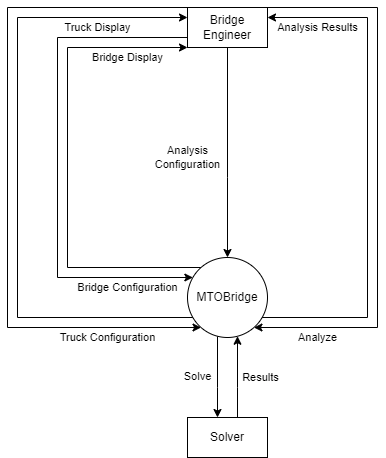
\includegraphics[]{context-diagram.png}
  \caption{Context Diagram of MTOBridge}
  \label {fig:context-diagram}
\end{figure}

\subsubsection{Work Partitioning}

\begin{table}[hp]
  \caption{Business Event List} \label{TblEventList}
  \begin{tabular}{p{0.33\textwidth} | p{0.33\textwidth} | p{0.33\textwidth}}
  \toprule
  \textbf{Event Name} & \textbf{Input/Output} & \textbf{Summary}\\
  \midrule
  Engineer enters truck configuration & IN: Truck configuration, OUT: Truck display & Record truck configuration, show truck visualization\\
  \midrule
  Engineer enters bridge configuration & IN: Bridge configuration, OUT: Bridge display & Record bridge configuration, show bridge visualization\\
  \midrule
  Engineer enters analysis configuration & IN: Analysis configuration & Record analysis configuration\\
  \midrule
  Engineer requests analysis & IN: Analyze request, OUT: Analysis results & Display analysis results\\
  \midrule
  Time to solve forces & OUT: Solve request, IN: Solver results & Give configurations to solver to get results\\
  \bottomrule
\end{tabular}
\end{table}

\subsubsection{Individual Product Use Cases}

\subsection{Functional Requirements}
  \textbf{FR.1} The Program should be able to call the backend MATLAB functions. \\
  \textbf{Rationale:} To visually display the outputs corresponding to user input, the UI needs to first figure out what those outputs are via the backend MATLAB.\\
  \textbf{Fit Criterion:} Realtively Binary, analyze whether or not the program can successfully call the MATLAB functions.\\\\
  
  \textbf{FR.2} The Program should allow the user to define the characteristics of the truck platoon, including truck configuration, number of trucks, headway, and travel speed.\\
  \textbf{Rationale:} The goal of the program is to determine the forces exerted by a given platoon on a bridge, they can come in many different forms, so flexibility in the characteristics
  of the platoon are necessary for the relevance of the simulation.\\ 
  \textbf{Fit Criterion:} At least one method of input(text based, dropdown list, etc) exists that allows users to specify those 4 characteristics of the platoon.\\\\

  \textbf{FR.3} The Program should allow the user to visualize the effects of their truck platoon characteristic definitions on the final platoon.\\
  \textbf{Rationale:} This is mainly to help the user verify that the inputs they put into the program correspond to the platoon they had in mind. As we are making a GUI,
  visual feedback is paramount to functionality.\\
  \textbf{Fit Criterion:} There exists some visual representation of the truck platoon that changes to reflect the impact of changes in user input.\\\\

  \textbf{FR.4} The Program should allow the user to define the characteristics of the bridge, inclduing what type of bridge it is and its length.\\
  \textbf{Rationale:} Different bridges will react to the same truck platoon differently, therefore specifiying the relevant characteristics of the bridge is necessary for
  the relevance of the simulation.\\
  \textbf{Fit Criterion} At least one method of input(text based, dropdown list, etc) exists that allows users to specify those 2 characteristics of the bridge.\\\\
  
  \textbf{FR.5} The Program should allow the user to visualize the effects of their bridge characteristic definitions on the final bridge.\\
  \textbf{Rationale:} This is mainly to help the user verify that the inputs they put into the program correspond to the bridge they had in mind. As we are making a GUI,
  visual feedback is paramount to functionality.\\
  \textbf{Fit Criterion:} There exists some visual representation of the bridge that changes to reflect the impact of changes in user input.\\\\ 

  \textbf{FR.6} The Program should allow the user to define which of the two solvers they are interested in using.\\
  \textbf{Rationale:} as the MATLAB backend can solve for both the demand on a concerned section as the platoon drives along, as well as for which section has the 
  highest maximum demand over the course of the whole trip, and these are very different pieces of info, allowing the user to determine which they are currently interested in 
  is important.\\
  \textbf{Fit Criterion:} At least one method of input(text based, dropdown list, etc) exists that allows the user to choose which solver they are would like to use.\\\\

  \textbf{FR.7} The Program should allow the user to define a section of concern on the bridge.\\
  \textbf{Rationale:} The first solver revolves around calculating the demand on a certain point along the bridge as the truck platoon drives over, specifying what point it is
  that we care about is necessray for this function.\\
  \textbf{Fit Criterion:} At least one method of input(text based, dropdown list, etc) exists that allows the user to determine a section of concern on the bridge.\\\\

  \textbf{FR.8} The Program should allow the user to define a discretization length for their bridge.\\
  \textbf{Rationale:} The second solver finds which section has the maximum demand placed on it over the course of the platoon's trip. The discretization length determines how
  many sections the bridge is split up into, which is necessary for the functioning of the second solver.\\
  \textbf{Fit Criterion:} At least one method of input(text based, dropdown list, etc) exists that allows the user to define a discretization length for their bridge.\\\\

  \textbf{FR.9} The Program should allow the user to define which type of demand placed on the bridge they are interested in, between shear forces and positive/negative moment.\\
  \textbf{Rationale:} There are a variety of different demands placed on the bridge as the platoon drives over, and the MATLAB backend contains calculations for all 3 of the
  above mentioned demands. Allowing the user to define which of the 3 they are interested in seeing is necessary for the functionality of the simulation.\\
  \textbf{Fit Criterion:} At least one method of input(text based, dropdown list, etc) exists that allows the user to define which of the 3 demands they are interested in
  simulating.\\\\

  \textbf{FR.10} The Program should be capable of visualizing the results of the concerned section calculation for the user.\\
  \textbf{Rationale:} This is essentially the main purpose of the GUI. Displaying the results of the MATLAB backend calculations visually to the user. This is one of the two
  main caluclations to be represented, so this functionality is very necessary.\\
  \textbf{Fit Criterion:} There exists some visualization of the mathematical results of the concerned section calculation.\\\\


\section{Non-functional Requirements}

\subsection{Look and Feel Requirements}

graphics (ui, animations, graphic element choice e.g. bridge mockup triangle/circle) will be informative, unobtrusive, and not distracting
rationale: no shit
fit criteria: reviewed by client contacts (civil engineers)?

\subsection{Usability and Humanity Requirements}

program will be intuitive to use
rationale: no shit
fit criteria: reviewed by civil engineers (our client contacts) to eliminate unintuitive controls?

program will have a user manual and (user-based) documentation provided
rationale: so that new people can actually use it quickly
fit criteria: they exist, idfk. review??

\subsection{Performance Requirements}

speed will be not unreasonably slow
rationale: no shit
fit criteria: ...program will not cause more than 1 second delay to any valid user input (independent of matlab component)?

precision reqs(!), program will be precise
rationale: no shit a bridge simulator should be precise
fit criteria: calculations are accurate to within (???)\% relative error of (other bridge simulation engine)

reliability and availability reqs? capacity reqs? probably N/A

\subsection{Operational and Environmental Requirements}

system/enviro constraints? if not a portability req

partner applications? if matlab integration not already mentioned

\subsection{Maintainability and Support Requirements}

portable for windows 10, distributable for standalone(!) use on windows 10
rationale: expected users dont all have matlab but will use windows 10
fit criteria: test it

\subsection{Security Requirements}

protect private mtobridge assets
rationale: why DO they not want their code uploaded anyway? ...confidentiality? why...?
fit criteria: don't upload them to the git my dude

\subsection{Cultural Requirements}

\subsection{Legal Requirements}

\subsection{Health and Safety Requirements}

This section is not in the original Volere template, but health and safety are
issues that should be considered for every engineering project.

\section{Project Issues}

\subsection{Open Issues}

\subsection{Off-the-Shelf Solutions}

\subsection{New Problems}

\subsection{Tasks}

\subsection{Migration to the New Product}

\subsection{Risks}

\subsection{Costs}

\subsection{User Documentation and Training}

\subsection{Waiting Room}

\subsection{Ideas for Solutions}

\newpage

\bibliographystyle {plainnat}
\bibliography {../../refs/References}

\newpage

\section{Appendix}

This section has been added to the Volere template.  This is where you can place
additional information.

\subsection{Symbolic Parameters}

The definition of the requirements will likely call for SYMBOLIC\_CONSTANTS.
Their values are defined in this section for easy maintenance.

\subsection{Reflection}

The information in this section will be used to evaluate the team members on the
graduate attribute of Lifelong Learning.  Please answer the following questions:

\begin{enumerate}
  \item What knowledge and skills will the team collectively need to acquire to
  successfully complete this capstone project?  Examples of possible knowledge
  to acquire include domain specific knowledge from the domain of your
  application, or software engineering knowledge, mechatronics knowledge or
  computer science knowledge.  Skills may be related to technology, or writing,
  or presentation, or team management, etc.  You should look to identify at
  least one item for each team member.
  \item For each of the knowledge areas and skills identified in the previous
  question, what are at least two approaches to acquiring the knowledge or
  mastering the skill?  Of the identified approaches, which will each team
  member pursue, and why did they make this choice?
\end{enumerate}

\end{document}